\section{Categorical Verification Results}

Categorical verification works quite well using the simple method describe in the the methdology.  Table~\ref{tab:type_class}
gives a summary of a pair of large traces with few categories.

\begin{table}[h]
\begin{center}
\begin{tabular}{| r | c | c | c |}
	\hline
	\textbf{Building} & \textbf{No. Sensors} & \textbf{No. Types} & \textbf{Accuracy}\\ \hline
	Todai & ~400 & 3 & 89\%    \\ \hline

	KETI & ~400 & 4 & 97\% 	 	\\ \hline

\end{tabular}
\caption{Categorical classification results for two data traces.}
\label{tab:type_class}
\end{center}
\end{table}

The simple methodology is able to separate them quite easily.  It is clear that the mean and standard deviation provides enough
inforomation for the classifier to differentiate between the different cateogories of traces.

% \begin{figure}[t!] %htbp
% \centering
% 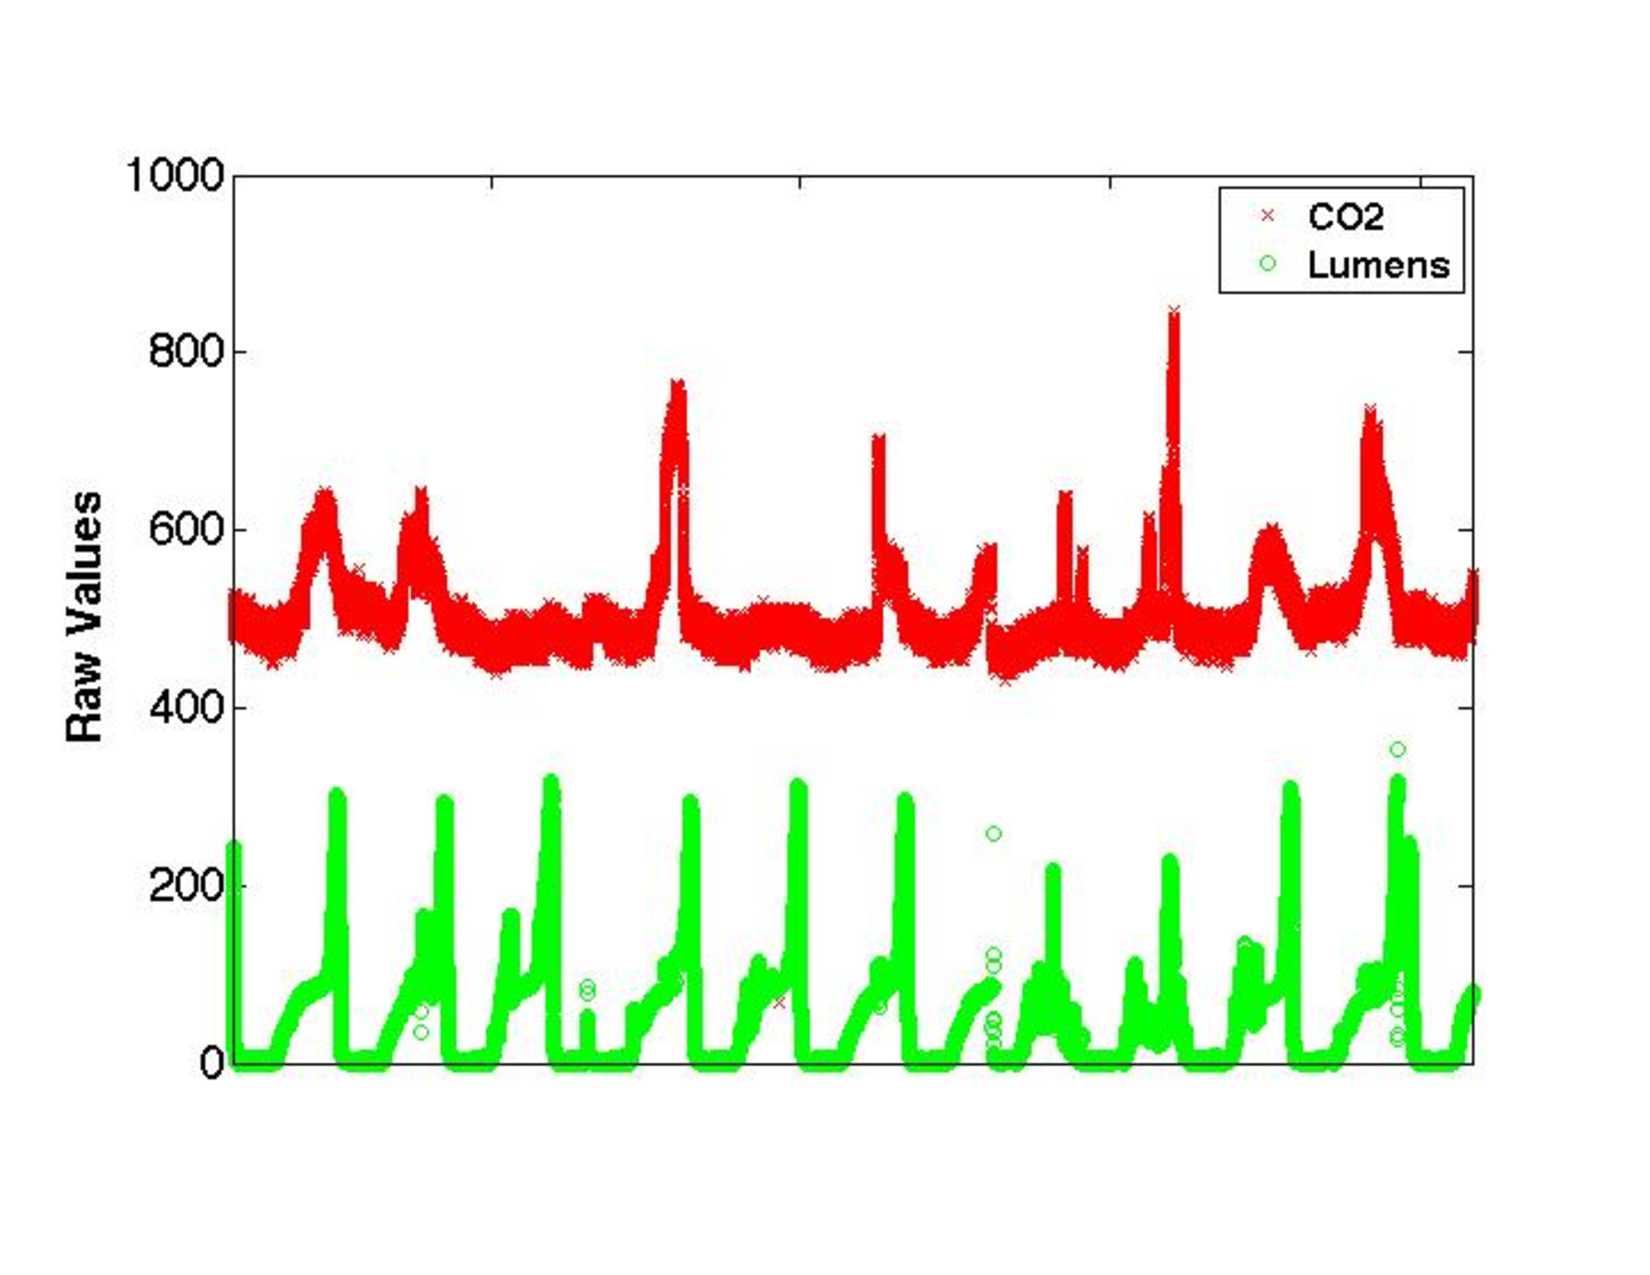
\includegraphics[width=0.75\columnwidth]{figs/KETI413_co2_light_raw}
% \caption{CO2 and Light traces from one of the rooms in Sutardja Dai Hall.  Note the values ranges and daily 
% fluctuations.}
% \label{fig:co2_light_raw}
% \end{figure}

% \begin{figure}[t!] %htbp
% \centering
% 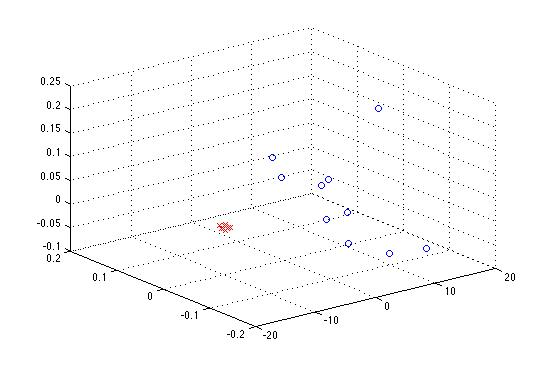
\includegraphics[width=0.75\columnwidth]{figs/EMD_LF_PCA_413_co2_light}
% \caption{CO2 and Light clusters.}
% \label{fig:EMD_LF_PCA}
% \end{figure}

% \begin{figure}[t!] %htbp
% \centering
% 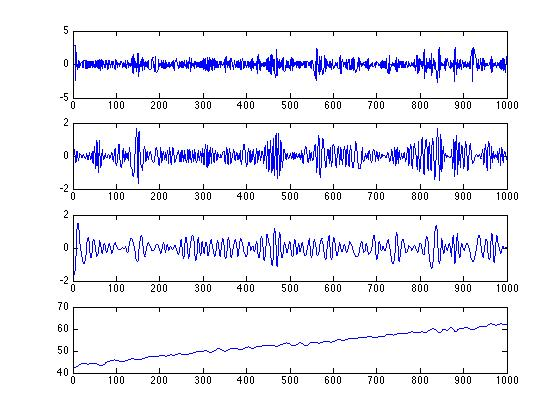
\includegraphics[width=0.75\columnwidth]{figs/KETI413_6h_light_3IMF}
% \caption{}
% \label{fig:light_3IMF}
% \end{figure}

% \begin{figure}[t!] %htbp
% \centering
% 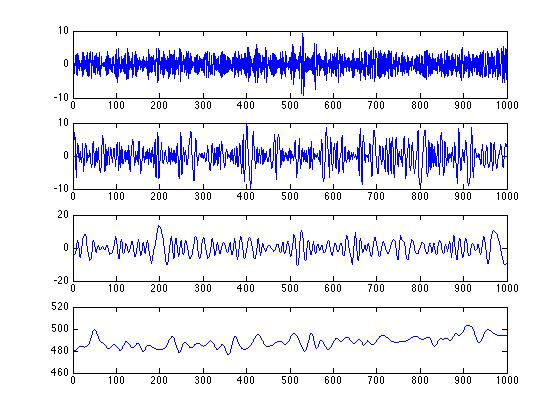
\includegraphics[width=0.75\columnwidth]{figs/KETI413_co2_6h_3IMFs}
% \caption{}
% \label{fig:co2_3IMFs}
% \end{figure}

The soda hall data traces were much more challenging to deal with. Soda hall was a much larger trace with 63 different
categorical tags on the traces.  Figure~\ref{fig:asovsagn} shows the AGN vs AGO cateogories.  Because the metadata for these is
not available, we do not have any semantic information about the meaning of the tags.  Note, there is a boundary between
mean values 3 and 4.

\begin{figure}[t!] %htbp
\centering
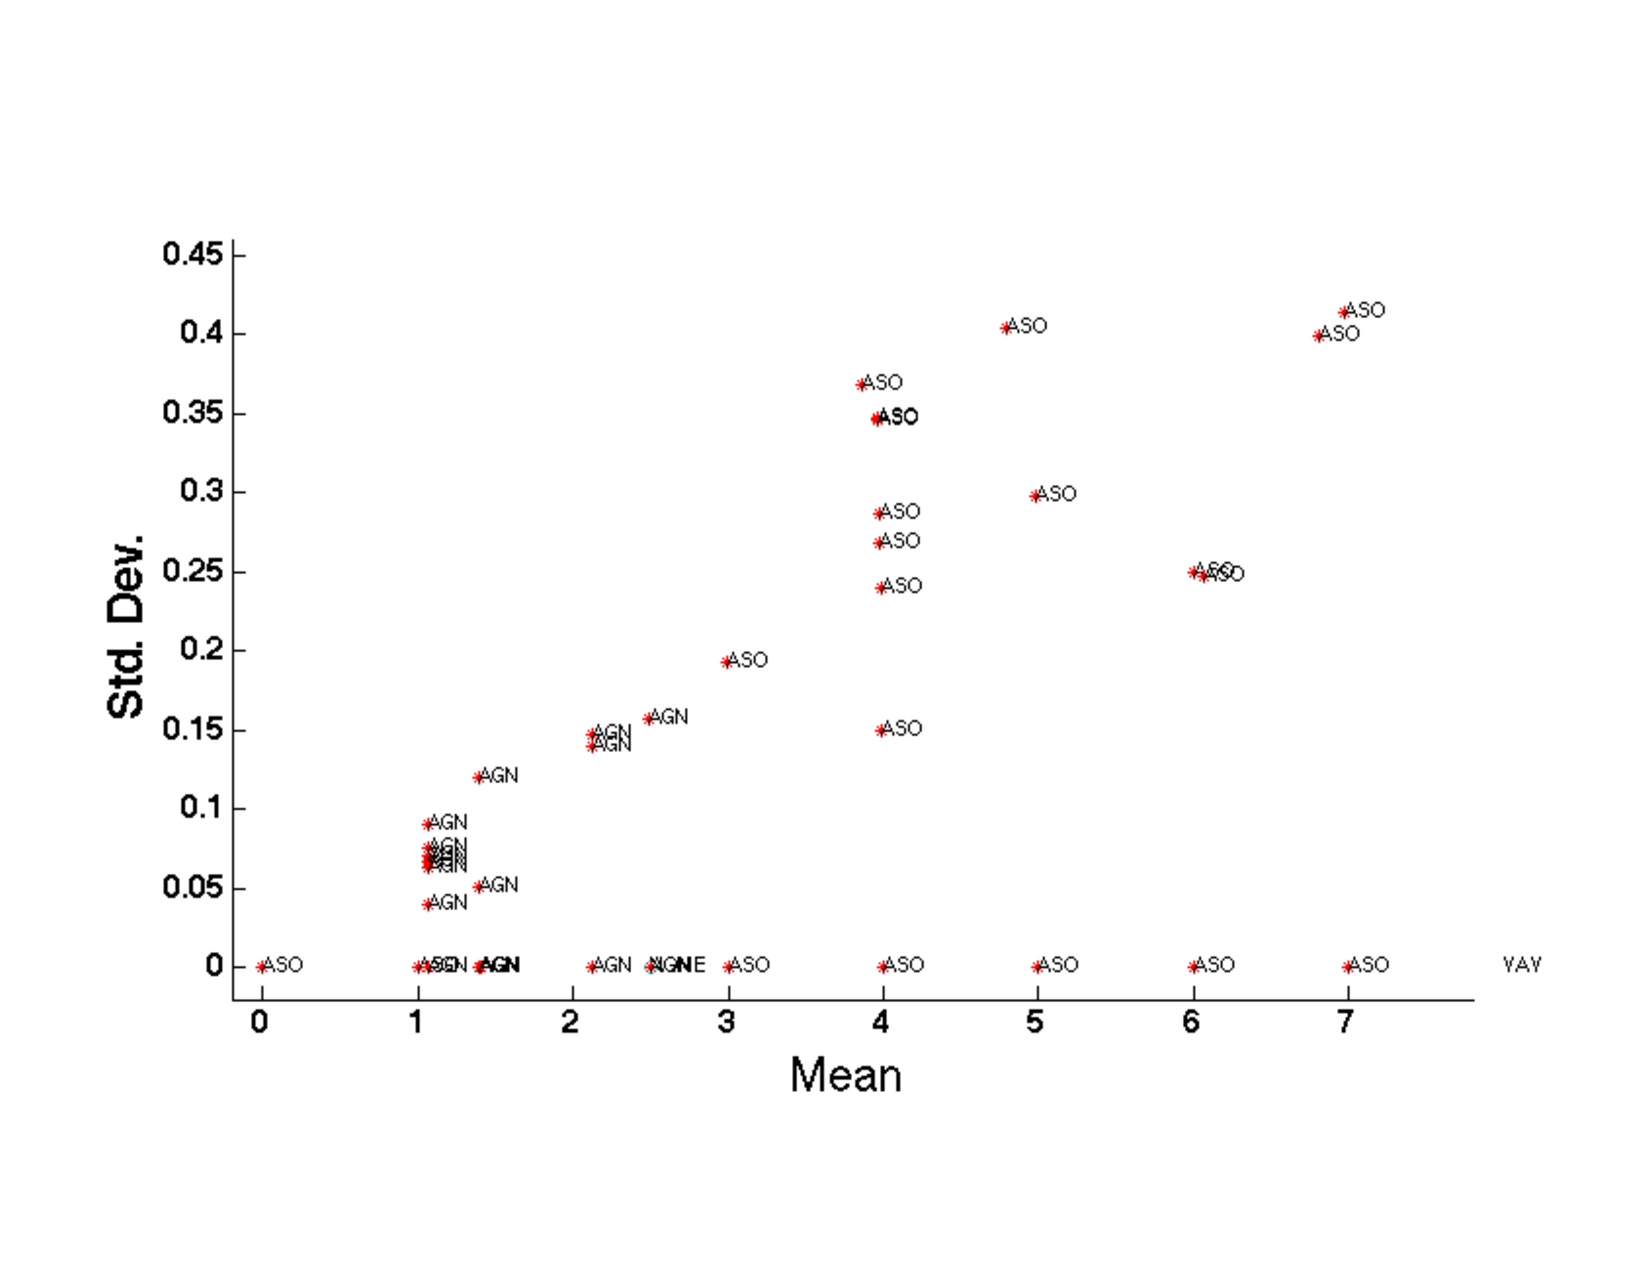
\includegraphics[width=0.8\columnwidth]{figs/ASOvsAGN}
\caption{ASO versus AGN.  There is a clear value-based boundary between the two sets of traces at around 3 in the mean.}
\label{fig:asovsagn}
\end{figure}

\begin{figure}[t!] %htbp
\centering
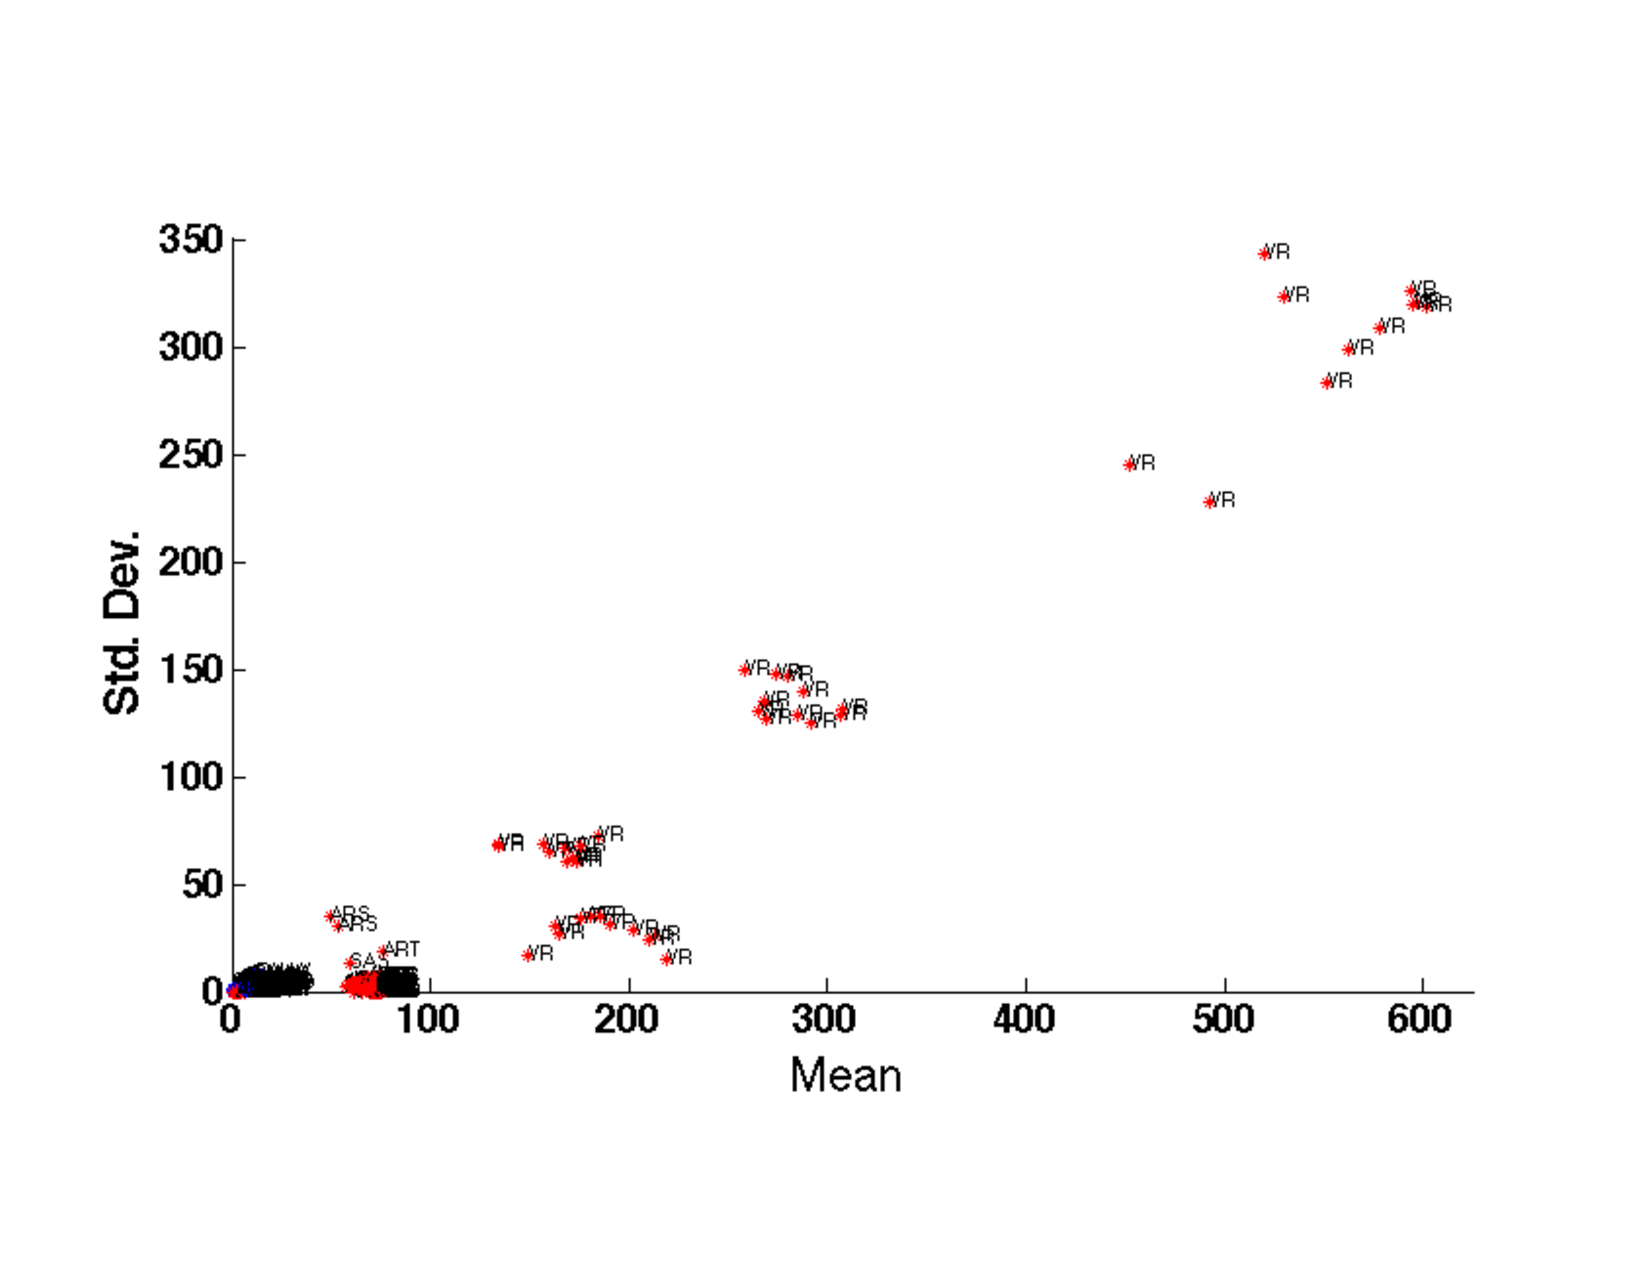
\includegraphics[width=0.8\columnwidth]{figs/VR}
\caption{The VR traces span a wide range, however, any mean above 100 is a VR trace.}
\label{fig:vr}
\end{figure}


% \begin{figure}[htb!]
% \begin{center}
% \subfloat[]{%
%             \label{fig:asovsagn}
%             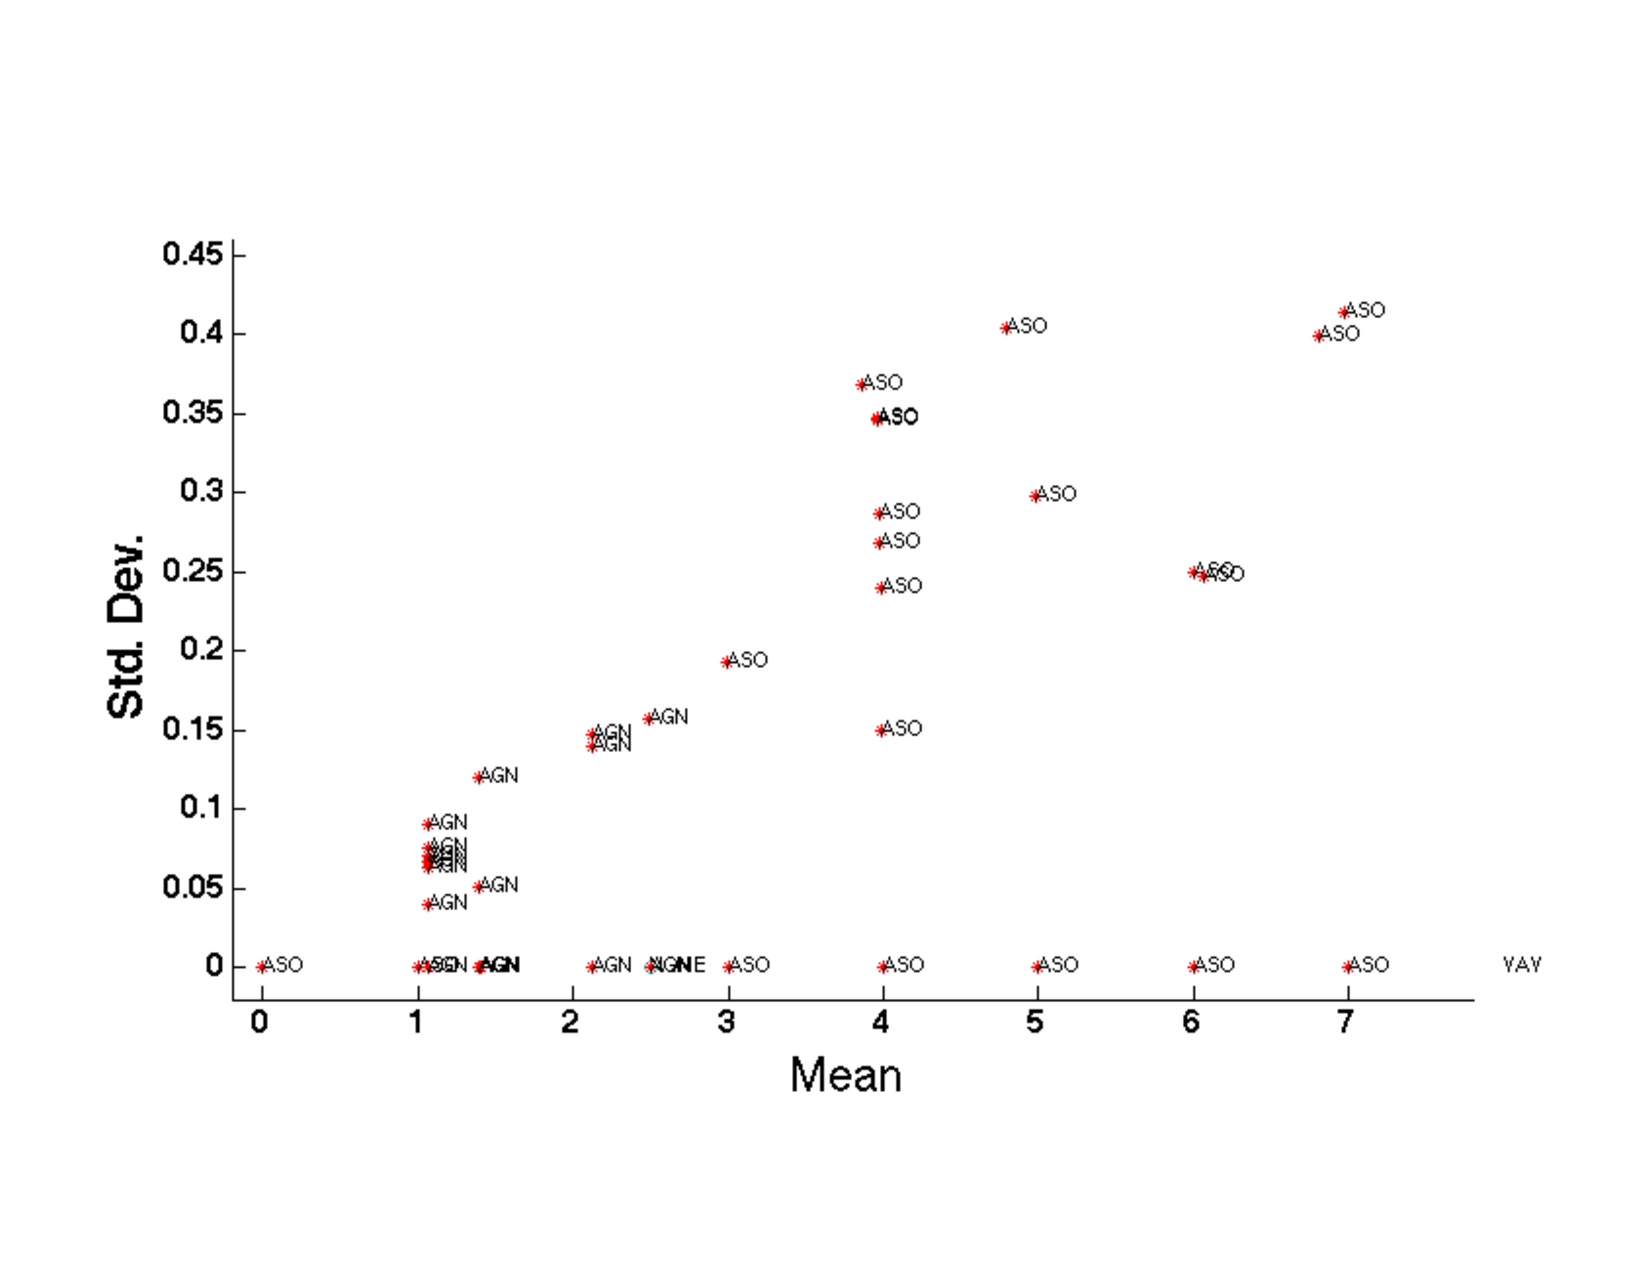
\includegraphics[scale=0.33]{figs/ASOvsAGN}
%         }
% \subfloat[]{%
%             \label{fig:vr}
%             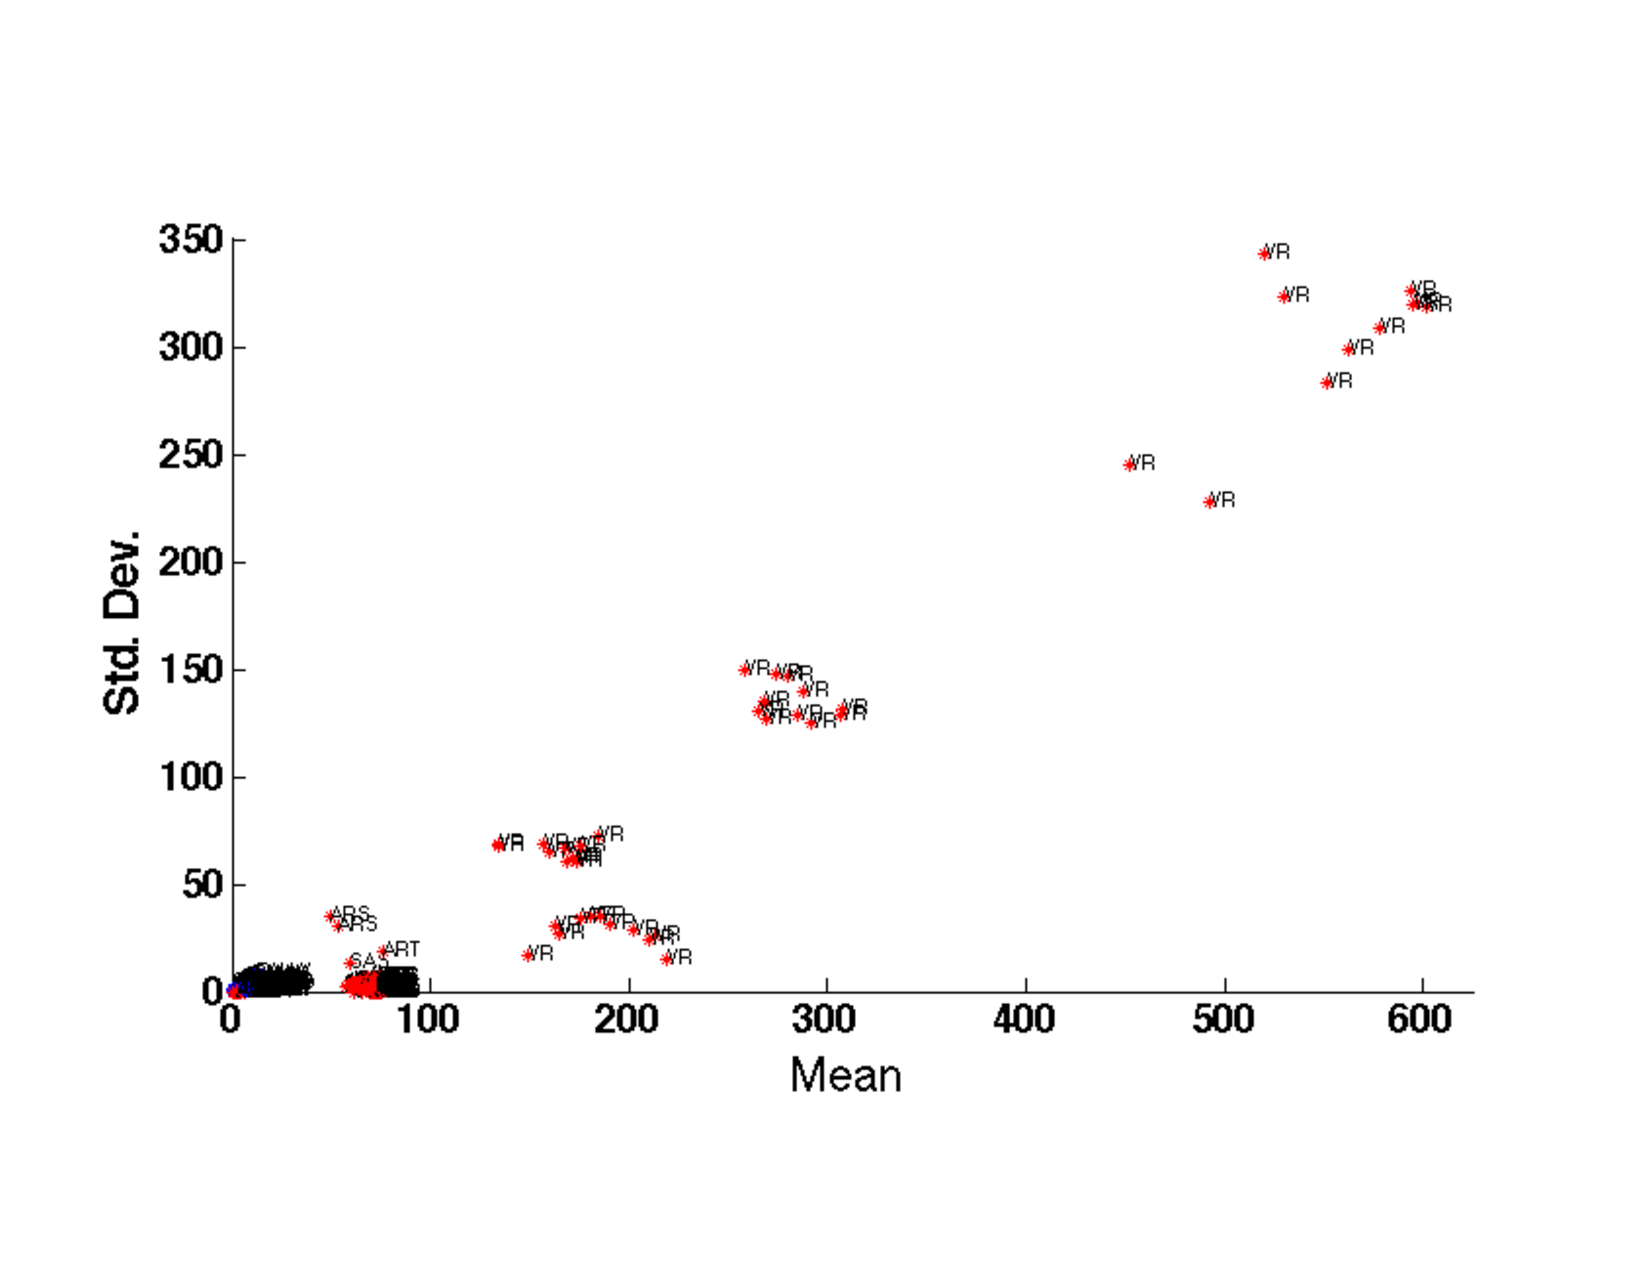
\includegraphics[scale=0.30]{figs/VR}
%         }
% \end{center}
% \caption{The figure on the left shows ASO and AGN traces.  There is a clear value-based boundary between the two sets of traces at around 3 in the mean.
% 	The figure on the right shows VR traces.  VR traces span a wide range, however, any mean above 100 is a VR trace.
%      }%
% \label{fig:agnagovr}
% \end{figure}

Our classifier was able to correctly classify the types with relatively few samples, giving us over 99\% classification accuracy in
the range presented in the the graph.  Similar results were obtained for separating the values presented in Figure~\ref{fig:vr}.
There is a clean boundary that is observable at around a mean value of 100.  Every trace with a mean greater than 100 was labeled as a VR
trace.  The accuracy is 100\%.

\begin{figure}[t!] %htbp
\centering
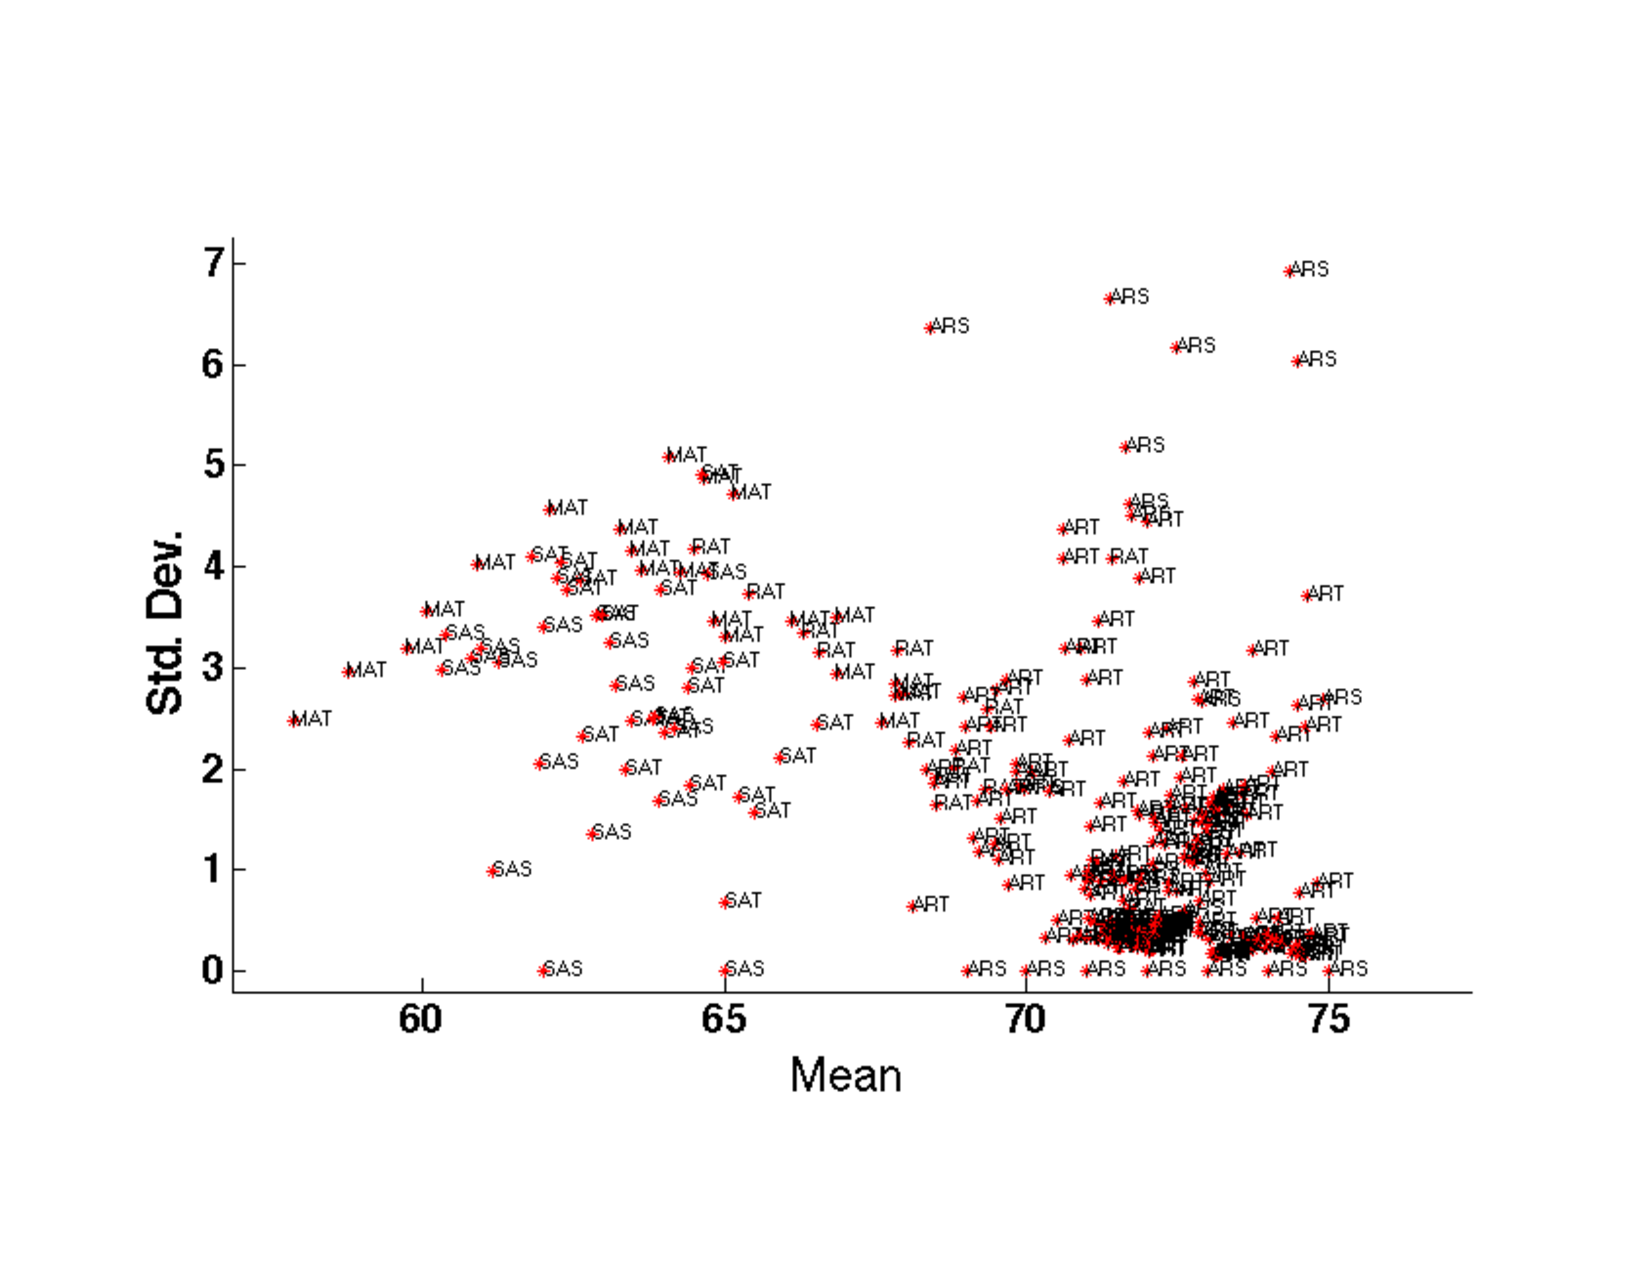
\includegraphics[width=0.8\columnwidth]{figs/temperature_streams}
\caption{All temperature streams.  Note, these are much more difficult to tease part.  A Gaussian mixture model can
separate them with approximately 77\% accuracy, but it may not generalize.}
\label{fig:temps}
\end{figure}

However, note the temperature traces between in Figure~\ref{fig:temps}.  The categorical clusters overlap signficantly.  We 
examined this distribution more closely by construct a Gaussia mixture model and plotting the cluster centers.  The results
are presented in Figure~\ref{fig:cluster_centers}.


\begin{figure}[t!] %htbp
\centering
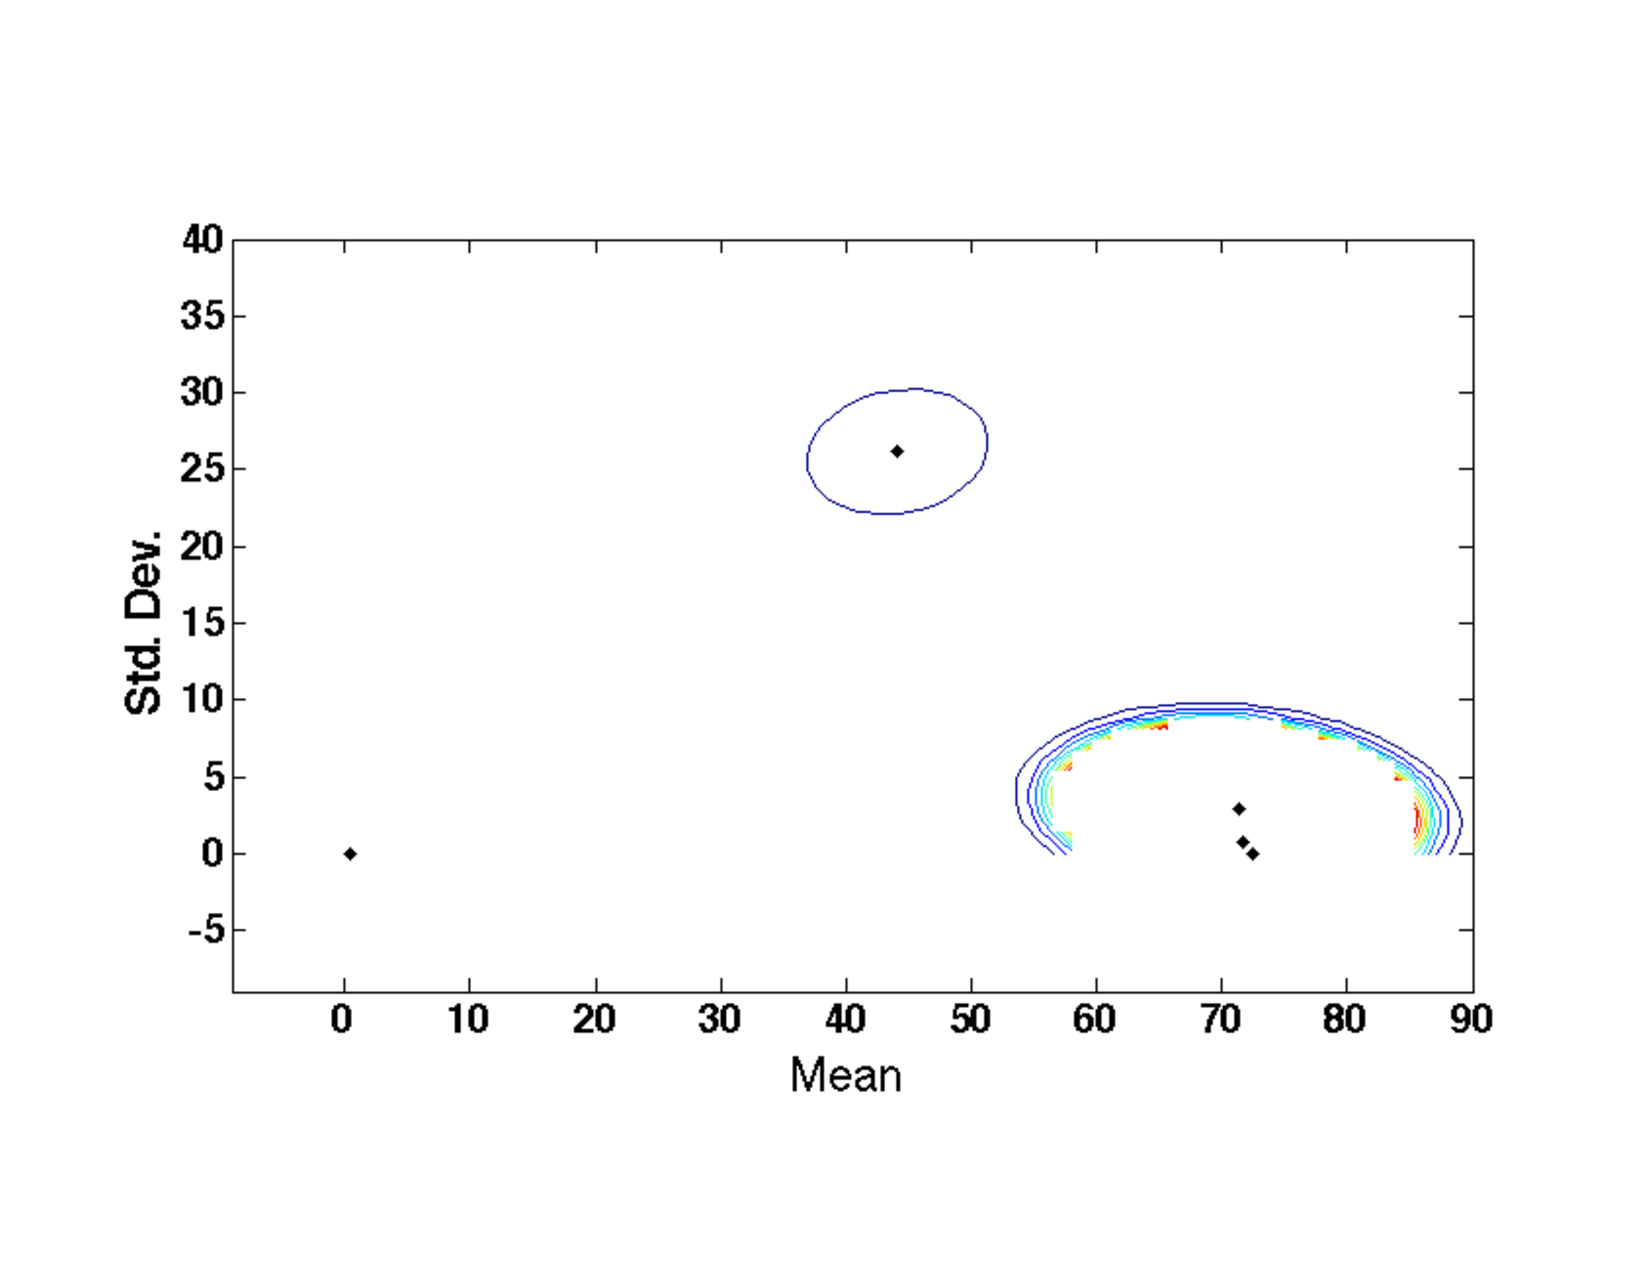
\includegraphics[width=0.8\columnwidth]{figs/gmm_centers}
\caption{Centers for our Gaussian mixture model.  Note, 3 of the 5 centers are very close to each other.  This makes these traces
very difficult tease apart and accurately classify.}
\label{fig:cluster_centers}
\end{figure}

Note, the cluster centers are not easily distinguishable.  The classifier varied in accuracy, leading us to believe that 
these sets of traces were mostly indistinguishable.  Moroever, our approach for this trace is very tightly tailored to
the particulars of this trace.  More exploration is necessary.



